\section{背景与动机}\label{sec:background}

\subsection{LLM 服务与 TTFT}

\begin{figure}[t!]
    \centering

    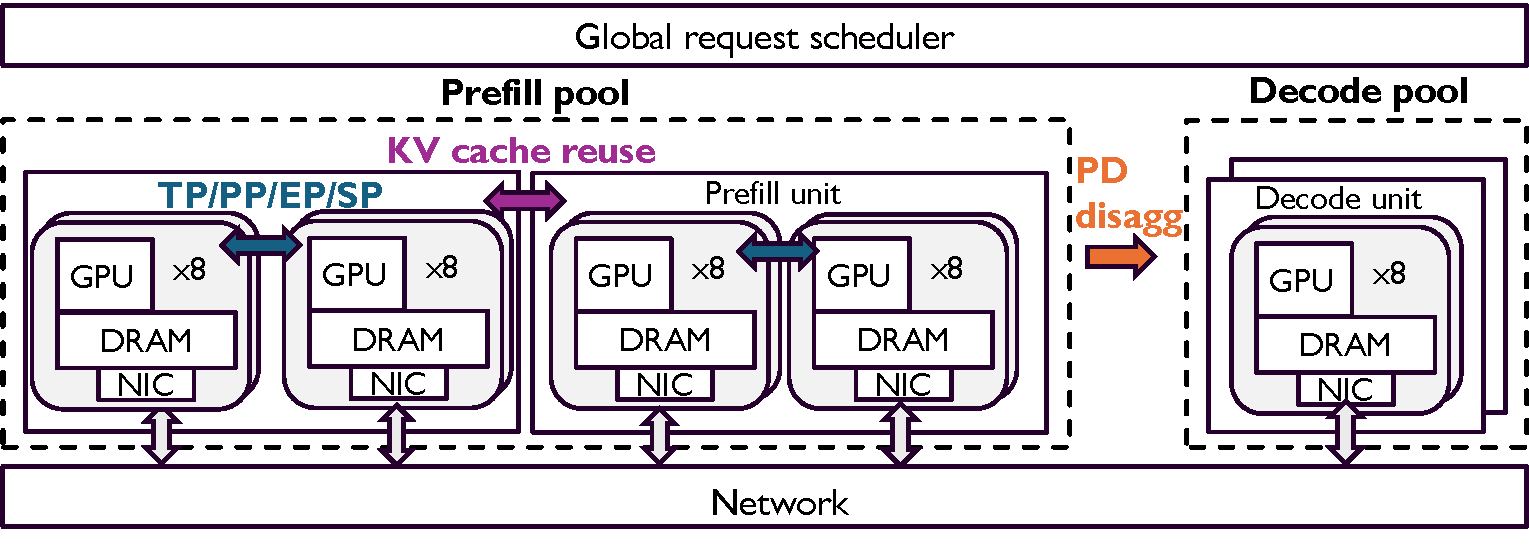
\includegraphics[width=\linewidth]{figures/moti/ServingOverview.pdf}
    \vspace{-0.5em}
    \caption{大规模 LLM 服务示意图。}
    \label{fig:bg:servingoverview}

\end{figure}


大型语言模型已经成为现代 AI 服务的基础。这类模型天然具有自回归特性：系统首先处理完整提示词以生成第一个 token（prefill 阶段），然后利用累积得到的 KV cache 迭代地产生后续 token（decode 阶段）。其性能通常用 prefill 阶段的首 Token 时间（TTFT）和解码阶段的 token 间时间（TBT）来刻画。

TTFT 是许多 LLM 应用中的关键服务级目标（SLO）。在聊天机器人、语音助手等交互式场景中，用户期望系统能够立即给出初始响应；一些研究表明，当延迟超过数百毫秒时，用户就会明显失去耐心，而达到数秒级则可能直接放弃~\cite{vijaya2025aqua,liu2025m,kim2025seconds}。TTFT 对自动化智能体框架同样重要，因为此类系统依赖严格超时~\cite{langfuse,LiteLLM}来实现容错。首个 token 延迟会触发代价高昂的补救动作，例如服务重试~\cite{Medium1,Medium2}或服务商切换~\cite{notdiamond}。微软近期的一份报告~\cite{ranganathan2025enhancing}显示，首个 token 延迟是服务失败（以超时报错形式体现）的主要来源之一（约占 40\%），并会带来收入损失、更高的支持成本和声誉风险。

如图~\ref{fig:bg:servingoverview} 所示，现代生产系统~\cite{mooncake,deepseektech}通常扩展到由数千个节点组成的集群，这些节点通过高带宽链路互连，每个节点内部包含多个 xPU（如 GPU、TPU、NPU）。节点被组织成独立的服务单元，每个单元承载一个模型副本。模型部署会结合张量并行~\cite{narayanan2021efficient}、流水线并行~\cite{narayanan2019pipedream, alphaserve}、序列并行~\cite{ringattention,wu2024loongserve,CP}和专家并行~\cite{expertparallel,deepspeedMoE,deepseektech,comet}等方式。为进一步提升效率，近期工作~\cite{distserve,splitwise,strati2024d,hu2024inference}提出\emph{prefill--decode 解耦}，将 prefill 任务部署在计算优化设备上，而将 decode 任务部署在内存更丰富的设备上，以适配其异构资源需求。此外，\emph{KV cache 复用}~\cite{mooncakefast,hu2024memserve,cachedattention,cacheblend}也被引入，通过在节点间迁移缓存上下文来摊薄 prefill 成本。

\begin{figure}[t!]
    \centering
    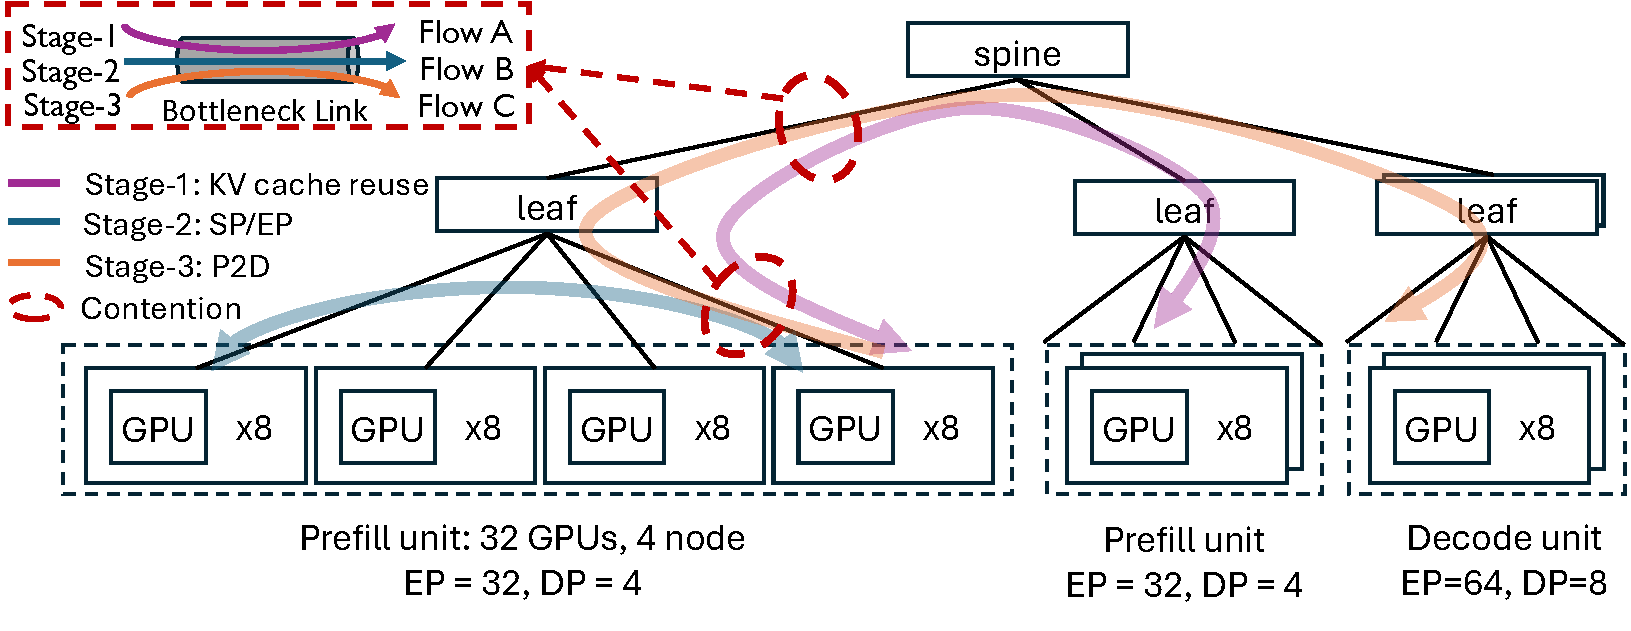
\includegraphics[width=\linewidth]{figures/moti/contentionmodel.pdf}
    \vspace{-0.5em}
\caption{LLM 服务系统中的通信争用示例：KV cache 传输（阶段 1 和 3）与并行通信（阶段 2）竞争同一链路带宽。}
    \label{fig:bg:contentionmodel}
\end{figure}

\begin{figure*}[ht!]
    \centering

    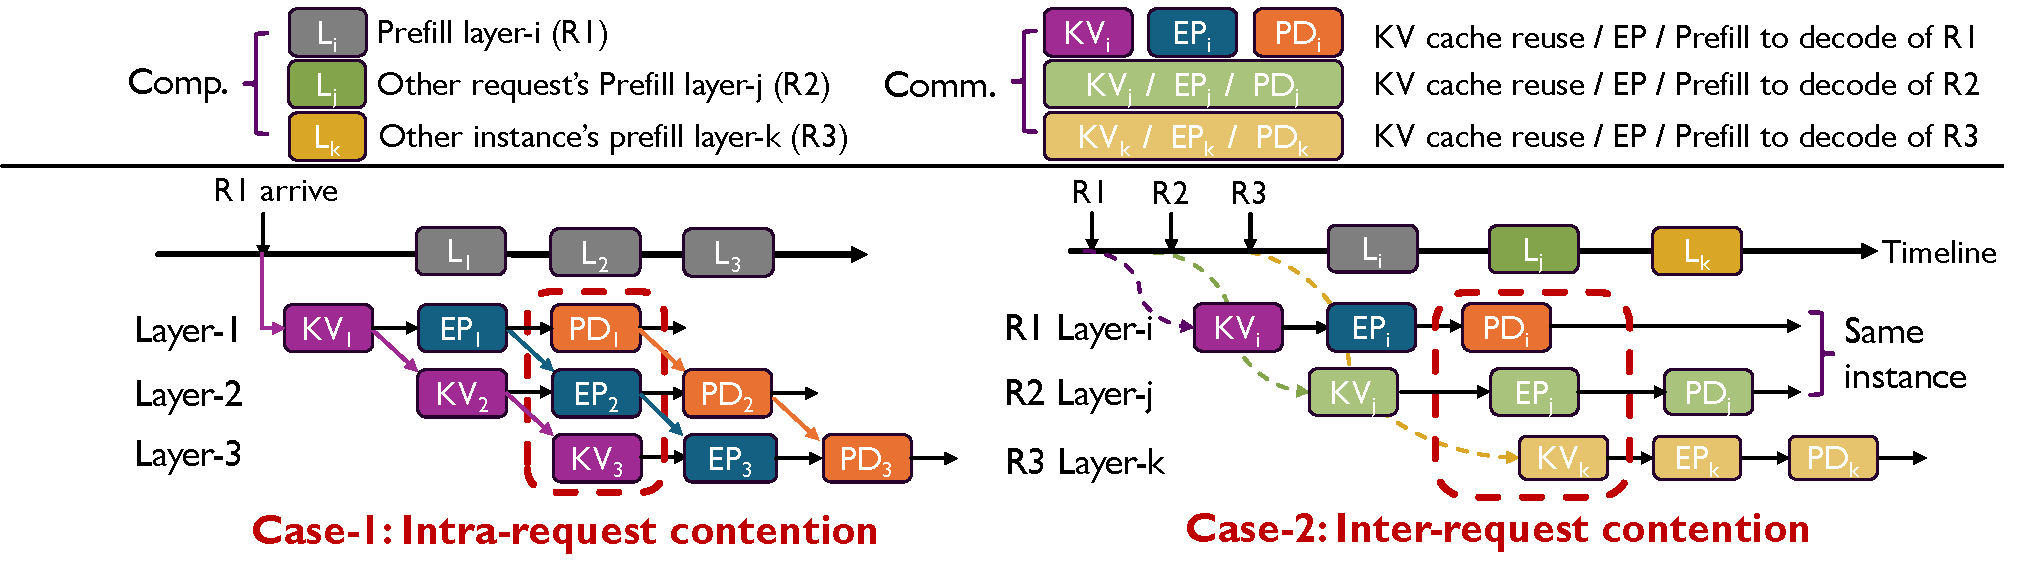
\includegraphics[width=0.9\linewidth]{figures/moti/contentioncase.pdf}

    \caption{LLM 服务系统中两类主要争用形式示意图。}
    \label{fig:bg:contention}
\end{figure*}


\subsection{多阶段通信中的争用}

在现有生产系统中生成第一个 token（图~\ref{fig:bg:servingoverview}）包含多阶段通信：
\begin{enumerate}[label=\(\bullet\),leftmargin=*]
    \item \textbf{阶段 1：KV-cache 复用}：从远端 prefill 单元拉取可复用的 KV-cache 块；
    \item \textbf{阶段 2：集合通信}：通过模型并行在设备间交换中间激活；
    \item \textbf{阶段 3：Prefill-to-Decode（P2D）传输}：将完整的 KV-cache 历史发送到 decode 单元\footnote{主流开源服务框架~\cite{vllm_pd_2025,sglang_pd_2025,dynamo_pd_2025}会显式地将阶段 3 的时延计入 TTFT 指标。}。
\end{enumerate}

已有文献指出，单个阶段本身就具有显著开销：集合通信（如 all-to-all 等）会占据端到端时延的 40--60\%~\cite{linaatc,comet,li2025optimizing,CP}，而 KV-cache 搬运也占据不可忽视的比例~\cite{cachegen,mooncake,chen2024kvdirect,li2025flowkv,yoon2025tract}。本文进一步识别出一个关键但研究不足的问题：集合通信与 KV-cache 搬运在时间上经常重叠，并竞争共享网络带宽。图~\ref{fig:bg:contentionmodel} 展示了争用在空间上的位置：KV-cache 传输（阶段 1 和 3）与集合通信（阶段 2）会经过相同的物理互连。这种空间共址造成了两类主要争用，如图~\ref{fig:bg:contention} 所示：
\begin{itemize}[leftmargin=*]
    \item \textbf{请求内争用}：单个请求内部不同通信流之间的相互干扰。具体来说，逐层的 KV-cache 传输（阶段 1 和 3）会与其他层正在进行的集合通信（阶段 2）直接竞争共享链路带宽。
    \item \textbf{请求间争用}：来自不同 prefill 单元的并发请求彼此干扰，导致交换机链路上频繁发生带宽竞争。此外，在块热门度分布倾斜的驱动下，多个 prefill 单元可能同时向同一个远端\textit{受害单元}拉取“热点”KV 块，从而在该受害单元的本地集合通信（阶段 2）与远程 KV-cache 拉取（阶段 1 和 3）之间，形成对其 NIC 带宽的竞争。
\end{itemize}

\begin{figure}[t]
    \centering
    \begin{subfigure}[t]{0.48\linewidth}
        \centering
        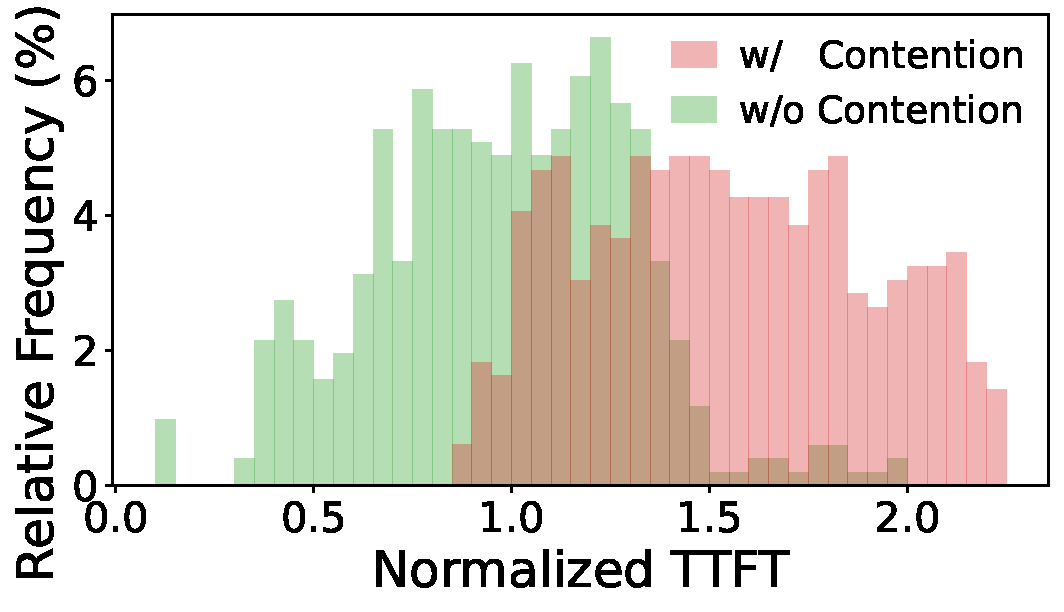
\includegraphics[width=\linewidth]{figures/moti/ttft_norm_hist_percent.pdf}
        \caption{争用对端到端 TTFT 的影响。}
        \label{fig:moti:ttft}
    \end{subfigure}
    \hfill
    \begin{subfigure}[t]{0.48\linewidth}
        \centering
        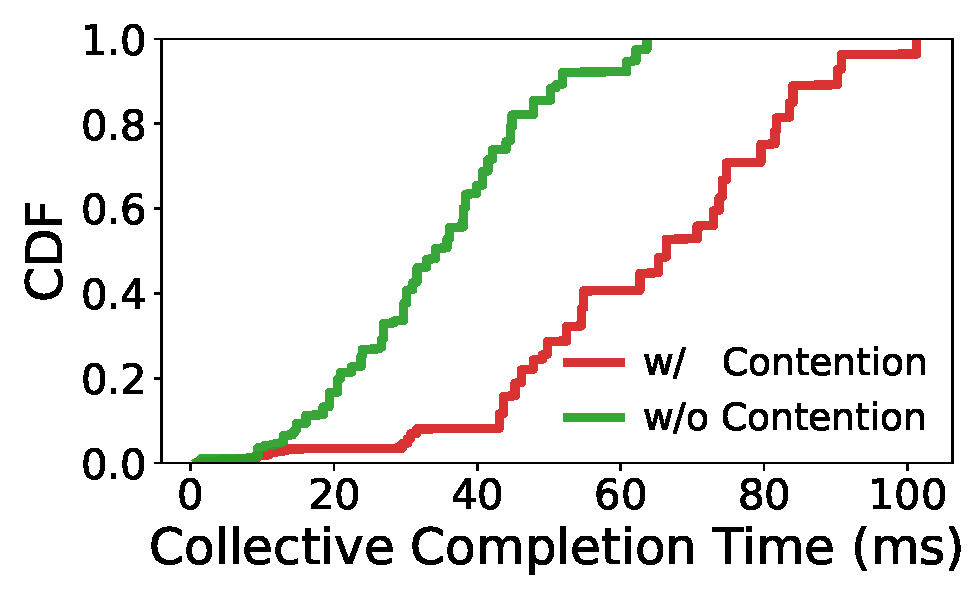
\includegraphics[width=\linewidth]{figures/moti/alltoall_8_cct_cdf.pdf}
        \caption{争用对 all-to-all 时延的影响。}
        \label{fig:moti:cct}
    \end{subfigure}
    \hfill

    \caption{【测试平台】通信争用对 Mixtral 8x7B 模型的影响。}

    \label{fig:moti:contentionimpact}
\end{figure}


为了量化这类干扰所带来的性能退化，我们在一个 16-GPU 的 prefill 集群（每 GPU 50 Gbps）上进行测量，集群中运行两个服务实例（$TP=1, EP=8$）。我们使用 QwenB-agent——一种来自生产环境 Qwen trace~\cite{qwen_bailian_traces} 的智能体工作负载，其平均序列长度为 1k token，prompt 复用率为 65\%，每 GPU 请求率为 1 req/s；完整测试平台设置见第~\ref{sec:evaluation:testbed} 节。我们评估争用对两个指标的影响：端到端 TTFT，以及 All-to-All 操作的集合通信时间（CCT，聚合 Dispatch 与 Combine 两阶段）。具体来说，我们比较理想基线（\textit{无争用}）与真实服务场景（\textit{有争用}）。图~\ref{fig:moti:ttft} 展示了 TTFT 分布。结果表明，在存在争用时，整体 TTFT 几乎被拉长了 50\%。我们将这一膨胀主要归因于关键路径上 All-to-All 通信时延的恶化：由于与并发 KV-cache 操作发生争用，其 CCT 几乎翻倍（$1.8\times$，见图~\ref{fig:moti:cct}）。这一显著减速证实，网络争用是 prefill 阶段性能波动的重要来源。

\subsection{现有工作的局限}
前述分析表明，缺乏管理的多阶段通信争用是 TTFT 违约的主要来源之一。我们将现有方法分为两类：近期的系统级通信优化，以及传统调度算法。如下所述，这两类方法都缺乏对多阶段依赖关系的整体视图，因此难以协调这类争用。

\parab{与阶段无关的流调度。} 传统数据中心调度策略以流或 coflow 为单位进行管理，优化的目标通常是流/协同流完成时间或截止期限满足率等网络指标。然而，这些目标与端到端应用目标（如 TTFT 达成率）并不一致，因为 TTFT 是由跨多个相互依赖阶段的流共同决定的。因此，这些方法不可避免地会过度优先松弛度较大的流，却让真正用于解锁下游计算的关键传输被饿死，最终恶化 TTFT SLO 达成率。

\parab{针对孤立阶段的专用优化。}
我们注意到，一些工作分别针对孤立阶段进行优化，具体包括：通过算法综合~\cite{shah2023taccl,liu2024rethinking,kim2024tccl,cao2025syccl}、参数调优~\cite{xu2025autoccl}和重叠执行~\cite{deepseektech,comet,zheng2025triton,zheng2025tilelink}来优化集合通信，或者通过流水线预取~\cite{splitwise,mooncakefast}和块合并~\cite{strati2024d,chen2024kvdirect,li2025flowkv}来优化 KV-cache 传输。然而，这些机制通常追求彼此冲突的目标。许多方法通过增加通信并发性来隐藏延迟，但没有一个机制能够在不同通信类型之间统一协调这种并发。结果是，即使引入了这些优化，集合通信和 KV-cache 传输仍常常彼此干扰，反而进一步放大争用。
